\documentclass[tikz,border=7pt]{standalone}
\usepackage{amsmath,pgfplots}
\pgfplotsset{compat=1.18}
\definecolor{ink}{HTML}{21352F}\definecolor{teal}{HTML}{087F7B}
\definecolor{gold}{HTML}{C58B2A}\definecolor{blue}{HTML}{4B77A8}\definecolor{rose}{HTML}{B65A62}
\begin{document}
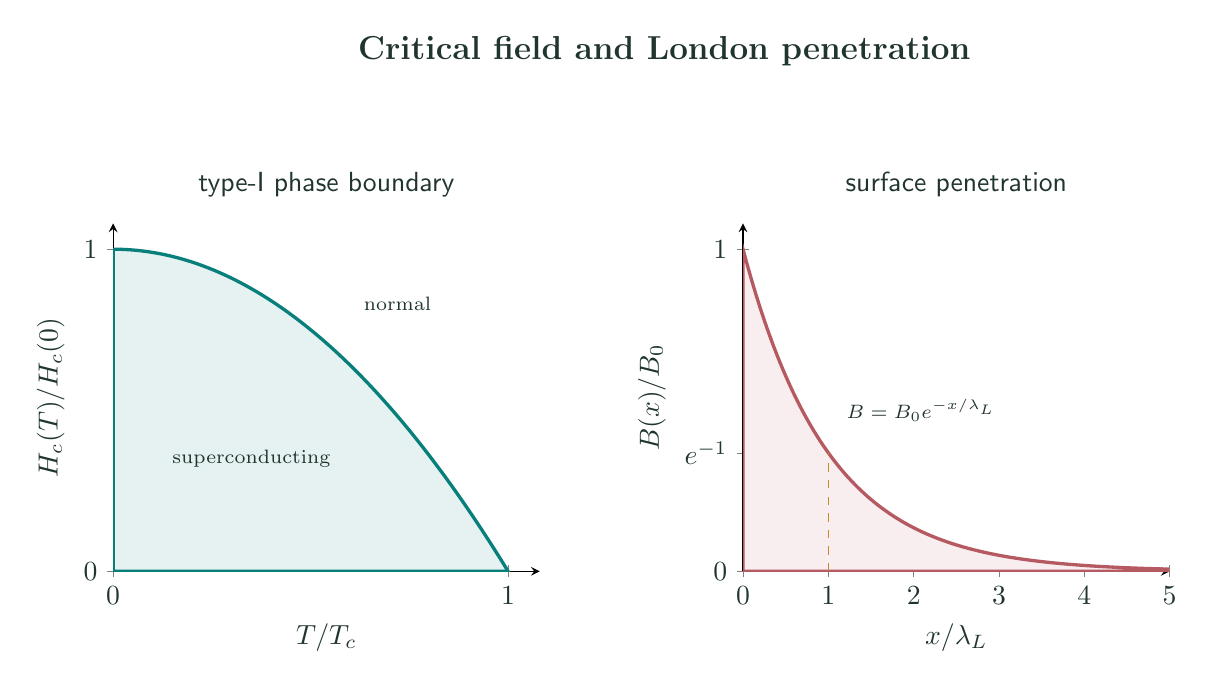
\begin{tikzpicture}[font=\sffamily,text=ink]
\node[font=\bfseries\large] at (0,3.8) {Critical field and London penetration};
\begin{axis}[at={(-7.0cm,-2.8cm)},anchor=south west,width=7cm,height=6cm,xmin=0,xmax=1.08,ymin=0,ymax=1.08,
 axis lines=left,xlabel={$T/T_c$},ylabel={$H_c(T)/H_c(0)$},xtick={0,1},ytick={0,1},title={type-I phase boundary}]
 \addplot[teal,very thick,domain=0:1,samples=180,fill=teal!10]{1-x^2}\closedcycle;
 \node[font=\scriptsize] at (axis cs:.35,.35) {superconducting};
 \node[font=\scriptsize] at (axis cs:.72,.83) {normal};
\end{axis}
\begin{axis}[at={(1.0cm,-2.8cm)},anchor=south west,width=7cm,height=6cm,xmin=0,xmax=5,ymin=0,ymax=1.08,
 axis lines=left,xlabel={$x/\lambda_L$},ylabel={$B(x)/B_0$},xtick={0,1,2,3,4,5},ytick={0,.368,1},yticklabels={$0$,$e^{-1}$,$1$},title={surface penetration}]
 \addplot[rose,very thick,domain=0:5,samples=180,fill=rose!10]{exp(-x)}\closedcycle;
 \draw[gold,dashed] (axis cs:1,0)--(axis cs:1,.368);
 \node[font=\scriptsize,anchor=west] at (axis cs:1.1,.5) {$B=B_0e^{-x/\lambda_L}$};
\end{axis}
\end{tikzpicture}
\end{document}
